% Options for packages loaded elsewhere
\PassOptionsToPackage{unicode}{hyperref}
\PassOptionsToPackage{hyphens}{url}
%
\documentclass[
]{article}
\usepackage{amsmath,amssymb}
\usepackage{lmodern}
\usepackage{iftex}
\ifPDFTeX
  \usepackage[T1]{fontenc}
  \usepackage[utf8]{inputenc}
  \usepackage{textcomp} % provide euro and other symbols
\else % if luatex or xetex
  \usepackage{unicode-math}
  \defaultfontfeatures{Scale=MatchLowercase}
  \defaultfontfeatures[\rmfamily]{Ligatures=TeX,Scale=1}
\fi
% Use upquote if available, for straight quotes in verbatim environments
\IfFileExists{upquote.sty}{\usepackage{upquote}}{}
\IfFileExists{microtype.sty}{% use microtype if available
  \usepackage[]{microtype}
  \UseMicrotypeSet[protrusion]{basicmath} % disable protrusion for tt fonts
}{}
\makeatletter
\@ifundefined{KOMAClassName}{% if non-KOMA class
  \IfFileExists{parskip.sty}{%
    \usepackage{parskip}
  }{% else
    \setlength{\parindent}{0pt}
    \setlength{\parskip}{6pt plus 2pt minus 1pt}}
}{% if KOMA class
  \KOMAoptions{parskip=half}}
\makeatother
\usepackage{xcolor}
\usepackage[margin=1in]{geometry}
\usepackage{listings}
\newcommand{\passthrough}[1]{#1}
\lstset{defaultdialect=[5.3]Lua}
\lstset{defaultdialect=[x86masm]Assembler}
\usepackage{graphicx}
\makeatletter
\def\maxwidth{\ifdim\Gin@nat@width>\linewidth\linewidth\else\Gin@nat@width\fi}
\def\maxheight{\ifdim\Gin@nat@height>\textheight\textheight\else\Gin@nat@height\fi}
\makeatother
% Scale images if necessary, so that they will not overflow the page
% margins by default, and it is still possible to overwrite the defaults
% using explicit options in \includegraphics[width, height, ...]{}
\setkeys{Gin}{width=\maxwidth,height=\maxheight,keepaspectratio}
% Set default figure placement to htbp
\makeatletter
\def\fps@figure{htbp}
\makeatother
\setlength{\emergencystretch}{3em} % prevent overfull lines
\providecommand{\tightlist}{%
  \setlength{\itemsep}{0pt}\setlength{\parskip}{0pt}}
\setcounter{secnumdepth}{5}
\lstset{
  breaklines=true
}
\ifLuaTeX
  \usepackage{selnolig}  % disable illegal ligatures
\fi
\IfFileExists{bookmark.sty}{\usepackage{bookmark}}{\usepackage{hyperref}}
\IfFileExists{xurl.sty}{\usepackage{xurl}}{} % add URL line breaks if available
\urlstyle{same} % disable monospaced font for URLs
\hypersetup{
  pdftitle={Reporte\_04},
  pdfauthor={Jessica Garcia, Manuel Rivera, Axel Rodriguez},
  hidelinks,
  pdfcreator={LaTeX via pandoc}}

\title{Reporte\_04}
\author{Jessica Garcia, Manuel Rivera, Axel Rodriguez}
\date{2023-03-03}

\begin{document}
\maketitle

{
\setcounter{tocdepth}{2}
\tableofcontents
}
\hypertarget{crear-plot-de-h3k36me3-visualization-of-human-h3k36me3-chip-data}{%
\section{\texorpdfstring{Crear plot de H3K36me3 (\emph{visualization of
Human H3K36me3 ChIP
data})}{Crear plot de H3K36me3 (visualization of Human H3K36me3 ChIP data)}}\label{crear-plot-de-h3k36me3-visualization-of-human-h3k36me3-chip-data}}

\begin{lstlisting}[language=bash]

# Copiar los archivos necesarios a una carpeta de trabajo propia asignada para esta tarea

cd /mnt/Timina/bioinfoII/data/deepTools
cp H3K36me3.bw /mnt/Timina/bioinfoII/jgarcia/Tarea03
cp Human38_genesGencodev39.bed /mnt/Timina/bioinfoII/jgarcia/Tarea03 

# Cargar módulos
module load deeptools/2.4.1

#Generar una matriz de 2000 x 2000 que contenga las puntuaciones por regiones del genoma y preparar un archivo intermedio para usarse con el comando plotHeatmap.
computeMatrix reference-point -S H3K36me3.bw -R Human38_genesGencodev39.bed --referencePoint center -a 2000 -b 2000 -out matrix_H3K36me3_matrix.tab.gz

#Generar un mapa de calor para las puntuaciones asociadas a regiones genómicas
plotHeatmap -m matrix_H3K36me3_matrix.tab.gz -out H3K36me3_genes.png --heatmapHeight 15 --refPointLabel gene.center --regionsLabel genes --plotTitle ' H3K36me3 signal'
\end{lstlisting}

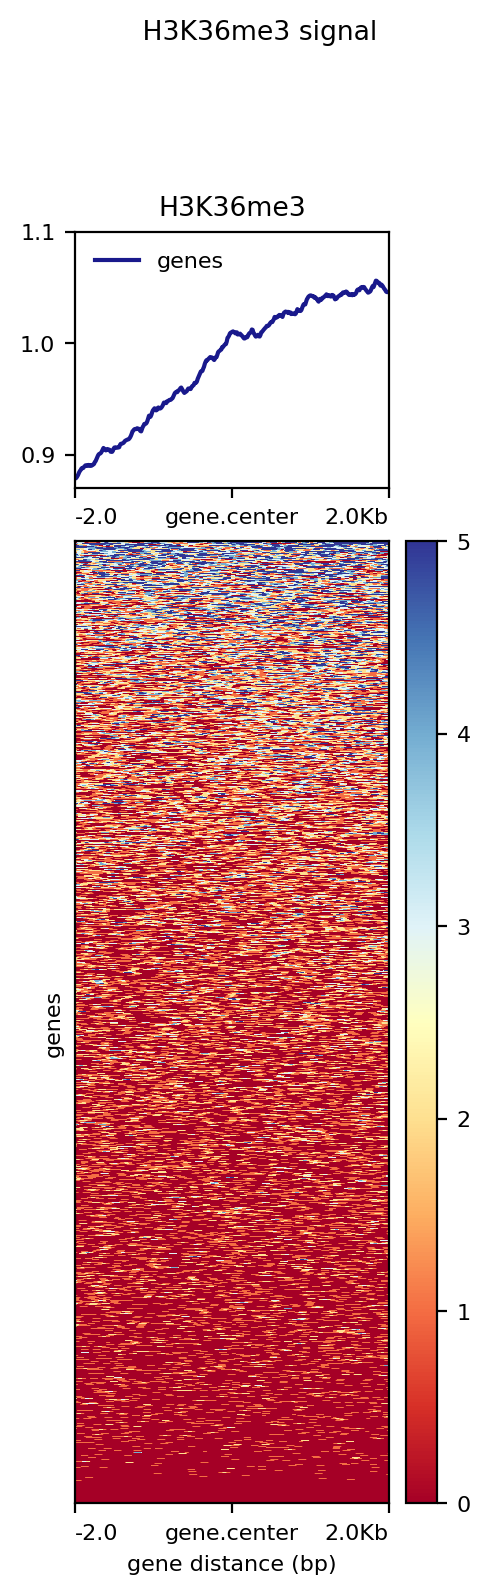
\includegraphics{./T04_images/H3K36me3_genes.png}

En esta imagen podemos observar en una región del centro de los genes a
-2.0 kb hasta 2.0 Kb que las señales de la histona H3K36me3 en los genes
humanos Gencodev39 no son lo suficientemente significativas, sin
embargo, podemos observar que hay una ligera señal aumentada en el sitio
terminal de la transcripción, al igual que en el sitio de inicio de la
transcripción, pero en menor medida.

\hypertarget{heatmap-de-ratuxf3n-visualization-of-m.-musculus-cebpa-chip-data}{%
\section{\texorpdfstring{Heatmap de ratón (\emph{visualization of M.
musculus Cebpa ChIP
data})}{Heatmap de ratón (visualization of M. musculus Cebpa ChIP data)}}\label{heatmap-de-ratuxf3n-visualization-of-m.-musculus-cebpa-chip-data}}

Para este ejemplo, vamos a crear un mapa de calor a partir de los datos
ChIP-seq de la tarea anterior. Es necesario un fichero bigWig
(\passthrough{\lstinline!Mus\_alg\_sorted.bw!}) que contenga los datos
de cobertura del experimento y un fichero \passthrough{\lstinline!.bed!}
que contenga las regiones de interés. En este caso, no tenemos un
fichero \passthrough{\lstinline!.bed!} de referencia para ratón, pero es
posible obtener uno entrando en el
\emph{\href{https://genome.ucsc.edu/cgi-bin/hgTables}{Table Browser}}
del \emph{UCSC Genome Browser} y rellenando un formulario de la
siguiente forma:

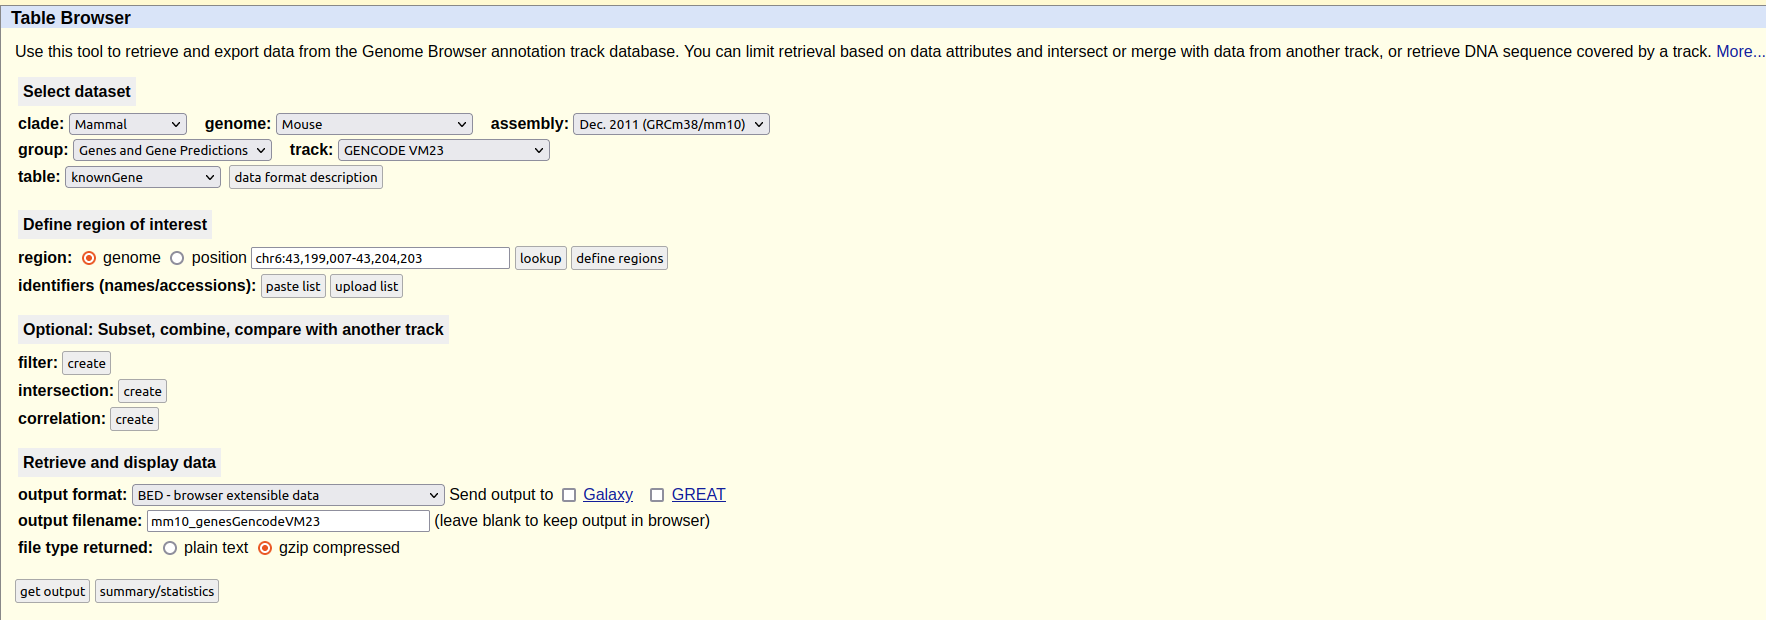
\includegraphics{./T04_images/TableBrowser.png}

Finalmente podemos elegir la opción de
\passthrough{\lstinline!Create one BED record per: Whole Gene!} y seguir
la descarga del archivo bed.

Posteriormente, para poder utilizar el archivo generado
(\passthrough{\lstinline!mm10\_genesGencodeVM23.gz!}) dentro del
cluster, se subió a Cyverse, generando un link de donde se puede
descargar. Para obtener el archivo se utilizó el siguiente comando:

\begin{lstlisting}[language=bash]
# Trabajando en /mnt/Timina/bioinfoII/arodriguez/Visualization
wget https://data.cyverse.org/dav-anon/iplant/home/axelrdz/Visualization/mm10_genesGencodeVM23.gz
\end{lstlisting}

Finalmente, se utilizó el archivo
\passthrough{\lstinline!HeatMapCEBPA.sge!} para generar el mapa de calor
que muestra la cobertura global del factor transcripcional de Cebpa en
el genoma de ratones para los datos de visualización generados en la
tarea anterior. El archivo contenia lo siquiente:

\begin{lstlisting}[language=bash]
#!/bin/bash
#
# Use Current working directory
#$ -cwd
#
# Join stdout and stderr
#$ -j n
#
# Run job through bash shell
#$ -S /bin/bash
#
# You can edit the script since this line
#
# Your job name
#$ -N HeatMapMusculusCenter
#
# Send an email after the job has finished
#$ -m e
#$ -M axelrdz5205@gmail.com
#
#
# If modules are needed, source modules environment (Do not delete the next line):
. /etc/profile.d/modules.sh
#
# Add any modules you might require:
module load deeptools/2.4.1
#
# Write your commands in the next line

# Trabajando en /mnt/Timina/bioinfoII/arodriguez/Visualization
# Computar la matriz
computeMatrix reference-point -S ./Mus_alg_sorted.bw -R ./mm10_genesGencodeVM23.bed -p max/2 --referencePoint TSS -a 2000 -b 2000 -out matrix_M_CEBPA_ChIP.tab.gz
\end{lstlisting}

\begin{itemize}
\tightlist
\item
  \passthrough{\lstinline!computeMatrix!} calcula puntuaciones por
  regiones genómicas y prepara un archivo intermedio que puede
  utilizarse con \passthrough{\lstinline!plotHeatmap!} y
  \passthrough{\lstinline!plotProfiles!}.
\item
  \passthrough{\lstinline!reference-point!} se refiere a una posición
  dentro de una región BED (por ejemplo, el punto de partida). En este
  modo, sólo se trazarán las posiciones genómicas antes
  (\passthrough{\lstinline!upstream!}) y/o después
  (\passthrough{\lstinline!downstream!}) del punto de referencia.
\item
  \passthrough{\lstinline!-S!}
  (\passthrough{\lstinline!--scoreFileName!}) es el archivo(s) bigWig
  que contiene los puntajes que se van a \emph{plotear}.
\item
  \passthrough{\lstinline!-R!}
  (\passthrough{\lstinline!--regionsFileName!}) es el nombre o nombres
  de archivos, en formato BED o GTF, que contienen las regiones a
  \emph{plotear}. Si se dan varios archivos BED, cada uno se considera
  un grupo que se puede trazar por separado.
\item
  \passthrough{\lstinline!-b!}
  (\passthrough{\lstinline!--beforeRegionStartLength!},
  \passthrough{\lstinline!--upstream!}) es la distancia \emph{upstream}
  del punto de partida de las regiones definidas en el archivo de región
  (\passthrough{\lstinline!mm10\_genesGencodeVM23.bed!}). Si las
  regiones son genes, esta sería la distancia \emph{upstream} del sitio
  de inicio de la transcripción. (Por defecto: 0).
\item
  \passthrough{\lstinline!-a!}
  (\passthrough{\lstinline!--afterRegionStartLength!},
  \passthrough{\lstinline!--downstream!}) es la distancia
  \emph{downstream} del punto final de las regiones dadas. Si las
  regiones son genes, esta sería la distancia aguas abajo del sitio
  final de la transcripción. (Por defecto: 0)
\item
  \passthrough{\lstinline!-out!}
  (\passthrough{\lstinline!--outFileName!},
  \passthrough{\lstinline!-o!}) es el nombre del archivo para guardar el
  fichero de la matriz computada.
\item
  \passthrough{\lstinline!-p max/2!} s para indicar que use la mitad del
  numero maximo de procesadores para acelerar el proceso
\end{itemize}

En un job aparte, se creo el archivo
\passthrough{\lstinline!CEBPA\_image.sge!}, que contena lo siguiente:

\begin{lstlisting}[language=bash]
#!/bin/bash
#
# Use Current working directory
#$ -cwd
#
# Join stdout and stderr
#$ -j n
#
# Run job through bash shell
#$ -S /bin/bash
#
# You can edit the script since this line
#
# Your job name
#$ -N CBPA_image
#
# Send an email after the job has finished
#$ -m e
#$ -M axelrdz5205@gmail.com
#
#
# If modules are needed, source modules environment (Do not delete the next line):
. /etc/profile.d/modules.sh
#
# Add any modules you might require:
module load deeptools/2.4.1
#
# Write your commands in the next line

# Trabajando en /mnt/Timina/bioinfoII/arodriguez/Visualization
# Crear Heatmap
plotHeatmap -m ./matrix_M_CEBPA_ChIP.tab.gz -out CEBPA_genes2.png --refPointLabel TSS --regionsLabel genes --plotTitle 'CEBPA signal'
\end{lstlisting}

\begin{itemize}
\tightlist
\item
  \passthrough{\lstinline!plotHeatmap!} crea un mapa de calor para las
  puntuaciones asociadas con regiones genómicas.
\item
  \passthrough{\lstinline!-m!} indica el archivo de matriz generado por
  la herramienta \passthrough{\lstinline!computeMatrix!}
  (\passthrough{\lstinline!matrix\_M\_CEBPA\_ChIP.tab.gz!}).
\item
  \passthrough{\lstinline!-out!} indica el nombre del archivo en el que
  guardar la imagen. La terminación del archivo se utilizará para
  determinar el formato de la imagen. Las opciones disponibles son:
  ``png'', ``eps'', ``pdf'' y ``svg''.
\item
  \passthrough{\lstinline!--refPointLabel!} es una etiqueta mostrada en
  el \emph{plot} para el punto de referencia. El valor predeterminado es
  el mismo que el punto de referencia seleccionado (p.~ej. TSS), pero
  podría ser cualquier cosa, p.~ej. ``peak start''.
\item
  \passthrough{\lstinline!--plotTitle!} es el título de la \emph{plot}.
\end{itemize}

\begin{lstlisting}[language=bash]
#Exportar a computadora local
rsync -rptuvl arodriguez@dna.lavis.unam.mx:/mnt/Timina/bioinfoII/arodriguez/Visualization/CEBPA_genes2.png .
\end{lstlisting}

\begin{center}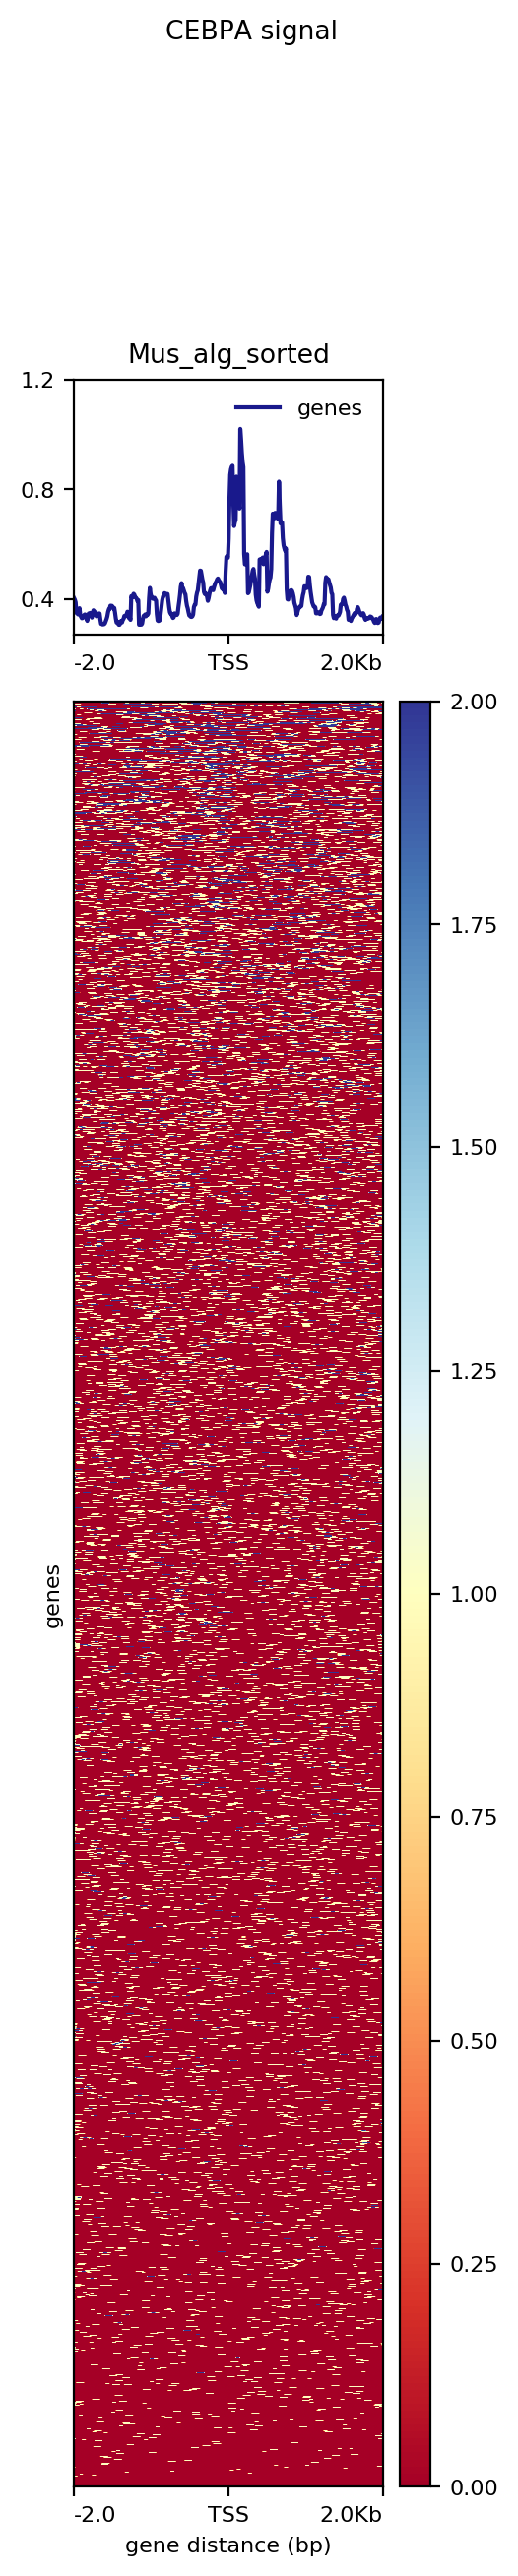
\includegraphics[width=300px]{./T04_images/CEBPA_genes2} \end{center}

Los datos se trazaron utilizando una matriz basada en puntos de
referencia centrada con una ventana de ± 2 kbp. Como se muestra en la
imagen, observamos un fuerte pico que marca el enriquecimiento de los
eventos de unión de Cebpa a la izquierda del centro del gen, hacia los
genes del inicio de la transcripcion, lo que estaría de acuerdo con su
naturaleza como factor de transcripción.

Cuando se observa el mapa de calor para la cobertura, sólo unos pocos
genes exhiben regiones azules. Estas regiones azules coinciden con las
regiones de ADN cercanas al sitio de inicio de la transcrcipción, lo
cual tiene sentido en este contexto. El que unos pocos genes exhiban
estas regiones azules se debe a que se tienen datos de CHIP-seq
hepáticos por lo que sólo los genes específicos del hígado exhibirán
estas regiones azules.

\hypertarget{visualizacion-de-histonas-h3k27me3-h3k36me3-h3k4me3}{%
\section{Visualizacion de Histonas H3K27me3, H3K36me3,
H3K4me3}\label{visualizacion-de-histonas-h3k27me3-h3k36me3-h3k4me3}}

\begin{lstlisting}[language=bash]
# Copiamos los archivos necesarios a nuestra carpeta
# Nota: trabajando en /mnt/Timina/bioinfoII/data/deepTools
cp H3K27me3.bw H3K36me3.bw H3K4me3.bw ../../arodriguez/Visualization/
# Visualizamos peso de los archivos
ls -lh
\end{lstlisting}

Teniendo en cuenta el tamaño de los archivos, la memoria disponible para
las sesiones de \passthrough{\lstinline!qlogin!} podría no ser
suficiente, y probablemente haría que el proceso se suspendiera
indefinidamente. Por lo tanto se generó un script sge llamadao
\passthrough{\lstinline!HistonesHeatmap4.sge!}, el cual contiene lo
siguiente:

\begin{lstlisting}[language=bash]
#!/bin/bash
#
# Use Current working directory
#$ -cwd
#
# Join stdout and stderr
#$ -j n
#
# Run job through bash shell
#$ -S /bin/bash
#
# You can edit the script since this line
#
# Your job name
#$ -N HistonesHeatmap4
#
# Send an email after the job has finished
#$ -m e
#$ -M axelrdz5205@gmail.com
#
#
# If modules are needed, source modules environment (Do not delete the next line):
. /etc/profile.d/modules.sh
#
# Add any modules you might require:
module load deeptools/2.4.1
#
# Write your commands in the next line

# Trabajando en /mnt/Timina/bioinfoII/arodriguez/Visualization
# Computar la matriz
computeMatrix scale-regions -S H3K27me3.bw H3K36me3.bw H3K4me3.bw -R Human38_genesGencodev39.bed --beforeRegionStartLength 1000 --regionBodyLength 1000 --afterRegionStartLength 1000 --skipZeros -o matrix.mat.gz
# Crear Heatmap
plotHeatmap -m matrix.mat.gz -out HistonesHeatmap.png --plotTitle 'Visualization of Human H3K27me3, H3K36me3, H3K4me3 ChIP data'
# Your job 274209 ("HistonesHeatmap4") has been submitted
\end{lstlisting}

\begin{lstlisting}[language=bash]
# Exportamos a computador local
rsync -rptuvl arodriguez@dna.lavis.unam.mx:/mnt/Timina/bioinfoII/arodriguez/Visualization/HistonesHeatmap.png .
\end{lstlisting}

\begin{center}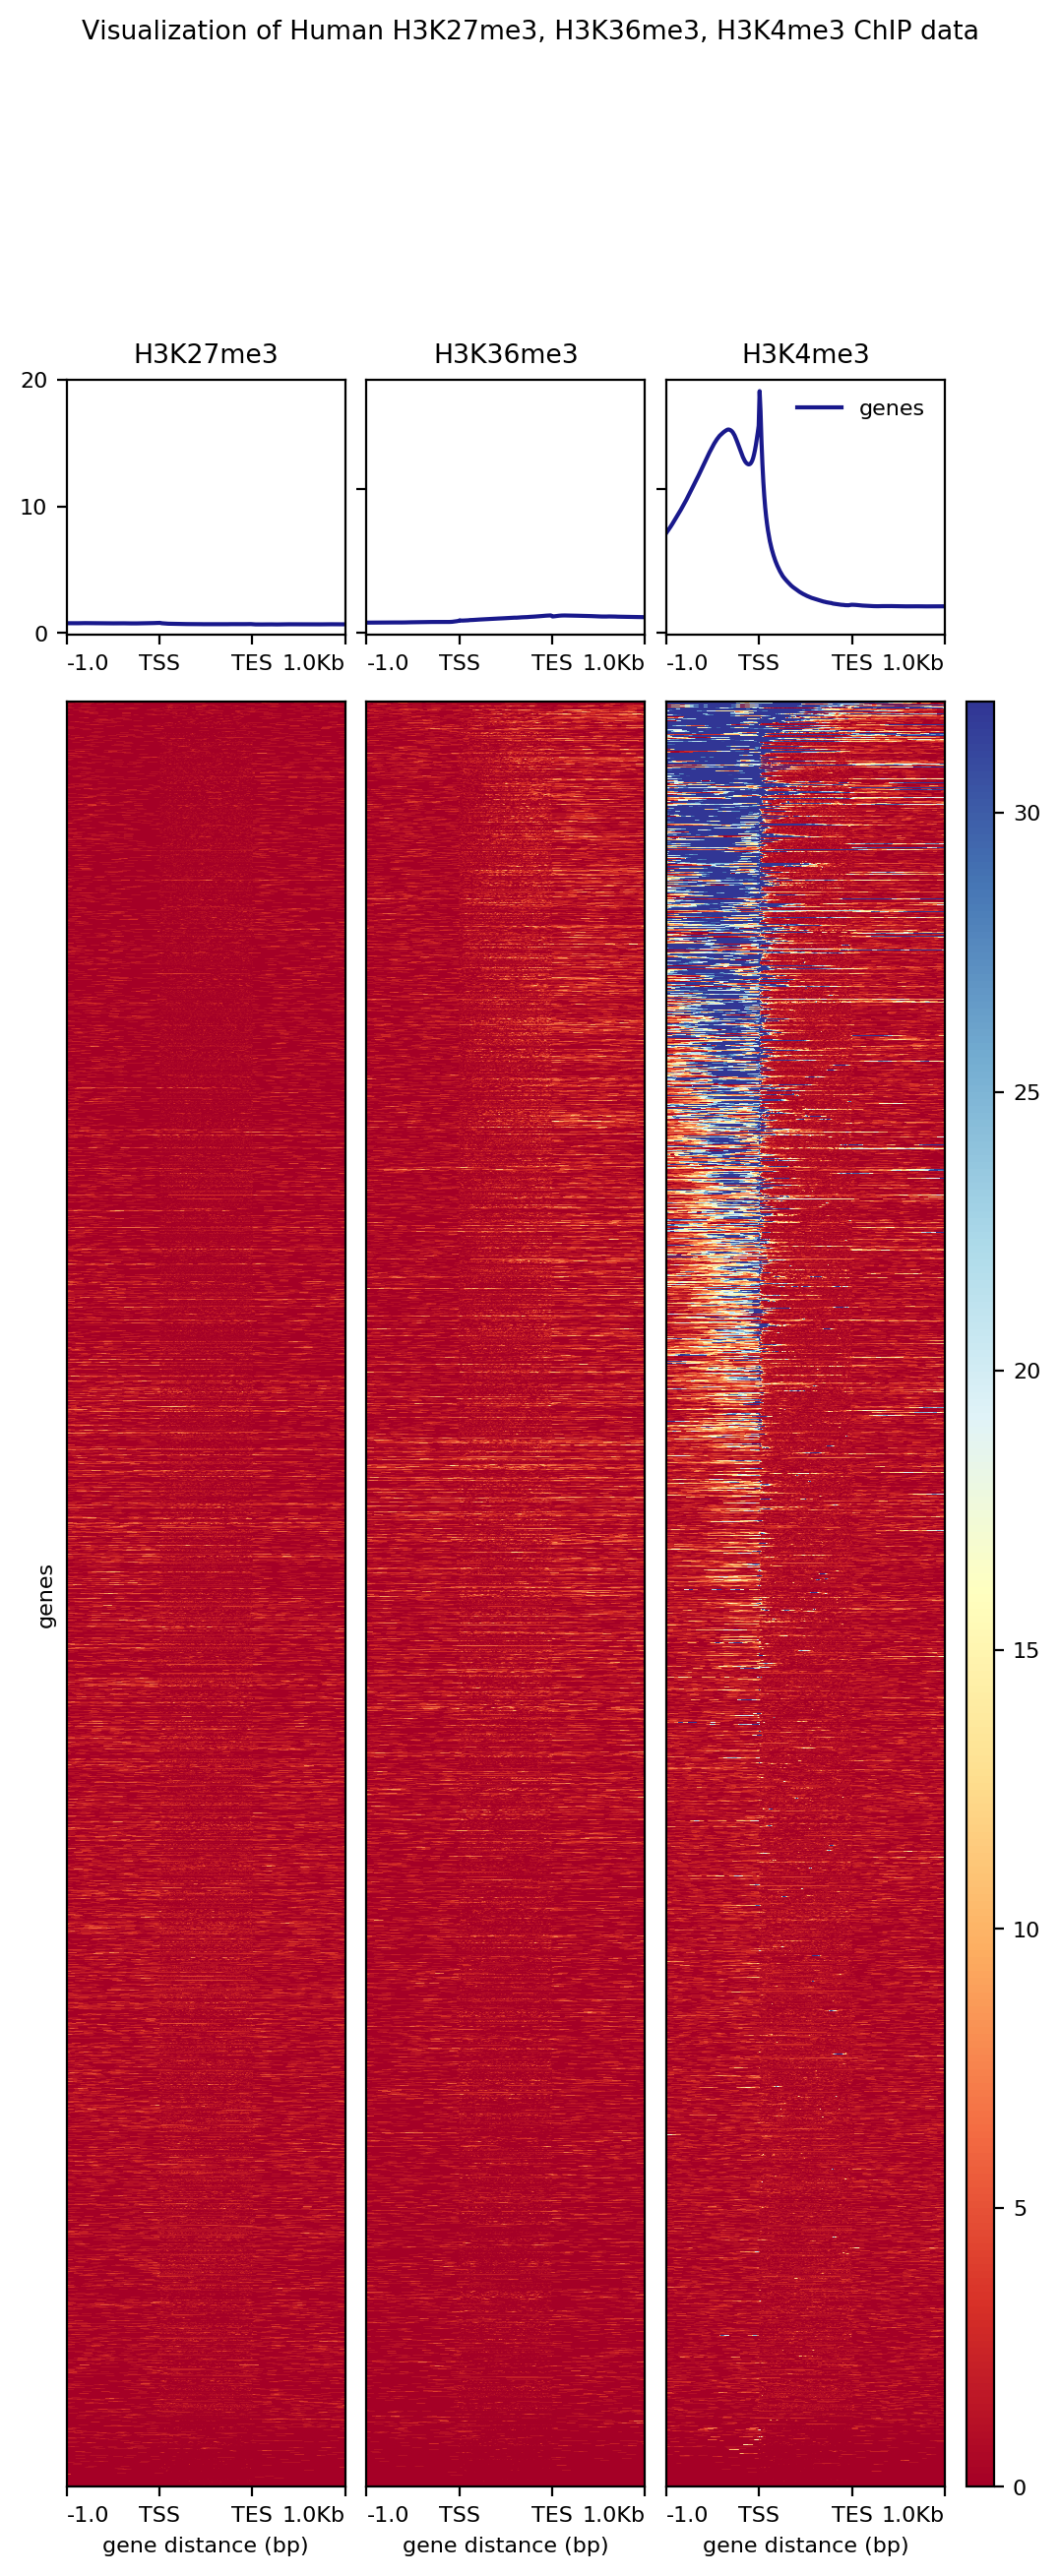
\includegraphics[width=600px]{./T04_images/HistonesHeatmap} \end{center}

Se produjo un gráfico comparativo entre los mapas térmicos de 3 histonas
diferentes, en este caso H3K36me del primer ejercicio, H3K27me que se
reportó como correlacionada con la represión de la cromatina y H3K4me3
que tiende a aparecer más frecuentemente cerca de los promotores y está
asociada a la transcripción. Con respecto al \emph{plot} anterior,
también se utilizaron \passthrough{\lstinline!scale-regions!} para
visualizar todos los genes normalizados a una determinada longitud.

Es posible apreciar una mayor detección de la señal de H3k4me3 cerca de
las secuencias promotoras de algunos genes, posiblemente indicando una
alteración positiva de la transcripción en estos genes donde la señal se
detecta a gran profundidad. H3K36me3 y H3K27me3 metilación no muestran
afinidad por una región particular de los genes o sus regiones
circundantes.

\hypertarget{tidytuesday-plot}{%
\section{`TidyTuesday plot'}\label{tidytuesday-plot}}

TidyTuesday plot. Elegir datos que le interesen y hacer una gráfica con
ellos

\begin{lstlisting}
## Rows: 195 Columns: 17
## -- Column specification --------------------------------------------------------
## Delimiter: ","
## chr  (3): Breed, Coat Type, Coat Length
## dbl (14): Affectionate With Family, Good With Young Children, Good With Othe...
## 
## i Use `spec()` to retrieve the full column specification for this data.
## i Specify the column types or set `show_col_types = FALSE` to quiet this message.
## Rows: 195 Columns: 11
## -- Column specification --------------------------------------------------------
## Delimiter: ","
## chr (3): Breed, links, Image
## dbl (8): 2013 Rank, 2014 Rank, 2015 Rank, 2016 Rank, 2017 Rank, 2018 Rank, 2...
## 
## i Use `spec()` to retrieve the full column specification for this data.
## i Specify the column types or set `show_col_types = FALSE` to quiet this message.
\end{lstlisting}

\begin{itemize}
\tightlist
\item
  Tratar como factor los datos no numericos. Hay algunos datos como la
  longitud del pelaje y el tipo de pelaje que no vienen en un factor
  numérico, por lo que los trate como factores (clases). También en el
  ranking hay razas que no tienen un ranking en algunos años, por lo que
  si no tienen ninguna posición les asigné el 0.
\end{itemize}

\begin{lstlisting}[language=R]
# Tratar como factor algunas variables
bt$`Coat Type` = as.factor(bt$`Coat Type`)
class(bt$`Coat Type`)

bt$`Coat Length` = as.factor(bt$`Coat Length`)
class(bt$`Coat Length`)

# Asignar a los valores sin ranking 0
br[is.na(br) ] = 0
\end{lstlisting}

\begin{itemize}
\tightlist
\item
  ¿Cómo saber que variables influyen en el posicionamiento del perro?
  Para esto utilizaré los datos más recientes, los del ranking de 2020,
  primero trataré de predecir que variables influyen en el
  posicionamiento de un perro, mediante una regresión logística.
\end{itemize}

Para ver las variables que tienen más significancia en el
posicionamiento me interesa observar el pvalor que muestra el `summary',
un menor pvalor es igual a mayor significancia.

\begin{lstlisting}[language=R]
# Remover columna con nombres de razas
bt = bt[,-1]

#Predecir que variables me importan
modelo = glm(br$`2020 Rank` ~ ., data=bt)
summary (modelo)
\end{lstlisting}

\begin{itemize}
\tightlist
\item
  Las variables que más influyen en la posición de un perro son:
  Playfulness Level, Coat Type( específicamente Plott Hounds) y Coat
  Grooming Frequency. Con estas variables generé un segundo modelo y
  también grafiqué el ranking de un perro contra el tipo de pelaje y la
  frecuencia de cepillado, ya que la frecuencia de cepillado y el tipo
  de pelaje son las variables que más influyen en la posición de una
  raza.
\end{itemize}

\begin{lstlisting}[language=R]
# Modelo con las variables que me importan
modelo2= glm(br$`2020 Rank` ~ bt$`Playfulness Level` + bt$`Coat Grooming Frequency` + bt$`Coat Type`)

#Generar grafica
library(ggplot2)
ggplot(mapping= aes(x=bt$`Coat Grooming Frequency`, y=br$`2020 Rank`, colour= bt$`Coat Type`))+ geom_point() + labs (y= "Ranking 2020", x = "Frecuencia de cepillado") + labs(color = "Tipo de pelo")
\end{lstlisting}

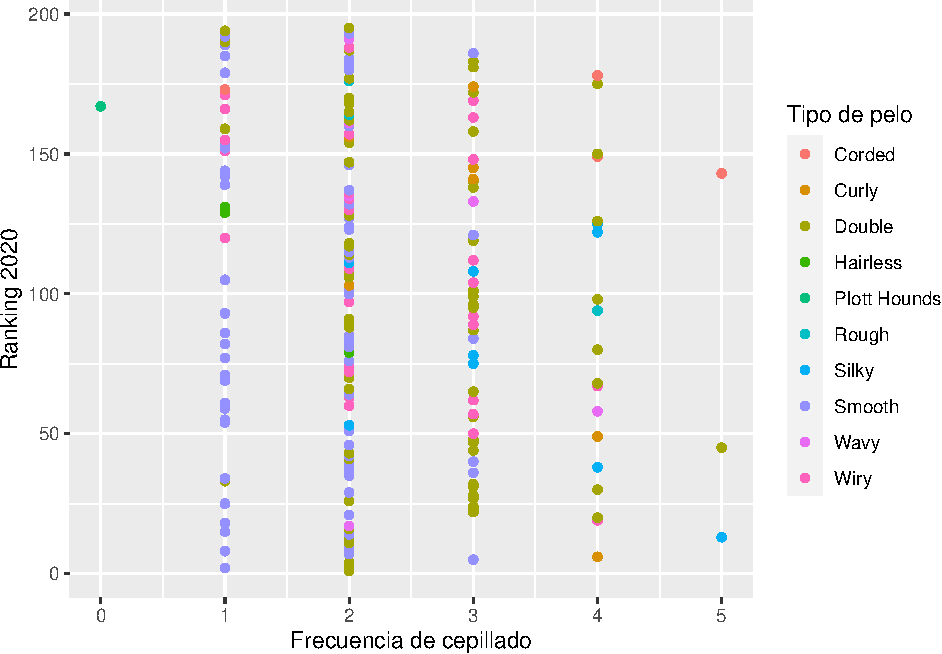
\includegraphics{Entrega04_files/figure-latex/unnamed-chunk-6-1.pdf}

\#Referencias

computeMatrix --- deepTools 3.5.0 documentation. (n.d.). Readthedocs.Io.
Recuperado Marzo 4, 2023, de
\url{https://deeptools.readthedocs.io/en/develop/content/tools/computeMatrix.html}

plotHeatmap --- deepTools 3.5.0 documentation. (n.d.). Readthedocs.Io.
Recuperado Marzo 4, 2023, de
\url{https://deeptools.readthedocs.io/en/develop/content/tools/plotHeatmap.html}

(N.d.). Nih.gov. Recuperado Marzo 4, 2023, de
\url{https://www.ncbi.nlm.nih.gov/pmc/articles/PMC6153486/}

\end{document}
